
\documentclass[10pt]{article}


\usepackage[colorlinks]{hyperref}


\usepackage{caption}
\usepackage[bottom]{footmisc}
\usepackage{float}
\usepackage{bm}
\usepackage{latexsym}
\usepackage{graphicx,wrapfig}
\usepackage[export]{adjustbox}
\usepackage{color}
\usepackage[dvipsnames]{xcolor}
\usepackage{verbatim}
\usepackage{array}
\usepackage{todonotes}
\usepackage{gensymb}
\usepackage{comment}
\usepackage[margin=0.7in]{geometry}
%\usepackage{ulem}
\usepackage[utf8]{inputenc}
\usepackage{amsmath}
\usepackage{subfigure}
\usepackage{microtype,xparse,tcolorbox}

\usepackage{hyperref}
\hypersetup{
	colorlinks=true,
	linkcolor=blue,
	filecolor=magenta,      
	urlcolor=blue,
}

\newcommand{\saha}[1]{\textcolor{magenta}{#1}}
\usepackage[T1]{fontenc}
\usepackage{titling}
\AtBeginDocument{\maketitle\thispagestyle{empty}\noindent}
\setlength{\droptitle}{-7em}
\title{Authors' cover letter for the revised version of document \textbf{JCAP\_101P\_0823} \\
	\vspace{-4ex}}

\date{\today}



\begin{document}
	\noindent\rule{18cm}{1pt}\\
	\textbf{Author(s)}: Sayan Saha, Louis Legrand, Julien Carron\\
	\textbf{Title}: Cluster profiles from  beyond-the-QE CMB lensing mass maps\\
	\noindent\rule{18cm}{1pt}\\
	
	This cover letter concerns our revision of the \textbf{JCAP\_101P\_0823} paper,
	entitled ``\textit{Cluster profiles from  beyond-the-QE CMB lensing mass maps}'', based on the referee's report. We first thank the referee for the insightful comments and suggestions about the paper. \\
	\\
	\textbf{Note:} We have kept the newly added or revised text in magenta colour in the revised draft, for convenience.
	
	\section{Response to the major comments}
	
	We have restructured the two subsections of section V, Results, with appropriate title as suggested. \\
	\\
	\textbf{Regarding the choice of different lmax and mass:} For the unlensed primodial CMB, and the Large scale structure (LSS) lensing field, the same set of Gaussian random fields has been used. For first subsection, the profile reconstruction, we wanted to show the dependendence of this bias on the mass in Fig. 3. Hence we have used a set of mass $M_{200}=4, 7$ and $10\times 10^{14} M_\odot$ for the results with simulations (along with the theoratical prediction).  In Fig. 2 we have shown the profile reconstruction with $M_{200}  = 4\times 10^{14} M_{\odot}$. On the other hand, to show the mass constraint in the second subsection, we choose $M_{200}=2\times 10^{14} M_{\odot}$. The reason behind such choice for the mass constraint is that this value (close to this value) is widely used to show the constraints, also most prabable value of mass in such redshift. Hence it will be conevenient to compare with other works in the literature. The reason, we choose a bit higher mass for Fig 2 and Fig. 4, is that we wanted to demonstrate how strongly the profile reconstruction gets bias when we use QE and how HDV QE and MAP estimator are in this context. We could use the same value, i.e. $M_{200}=2\times 10^{14} M_{\odot}$ but that wouldn't show us the bias in such prominent manner. Thank you for pointing this out. We have tried to revise the text to make the reason behind such choice clearer. The reason, behind taking lmax=5000, is also the same as the choice of higher lmax also enhances the amount of bias.    

\begin{figure}[H]
	\centering
		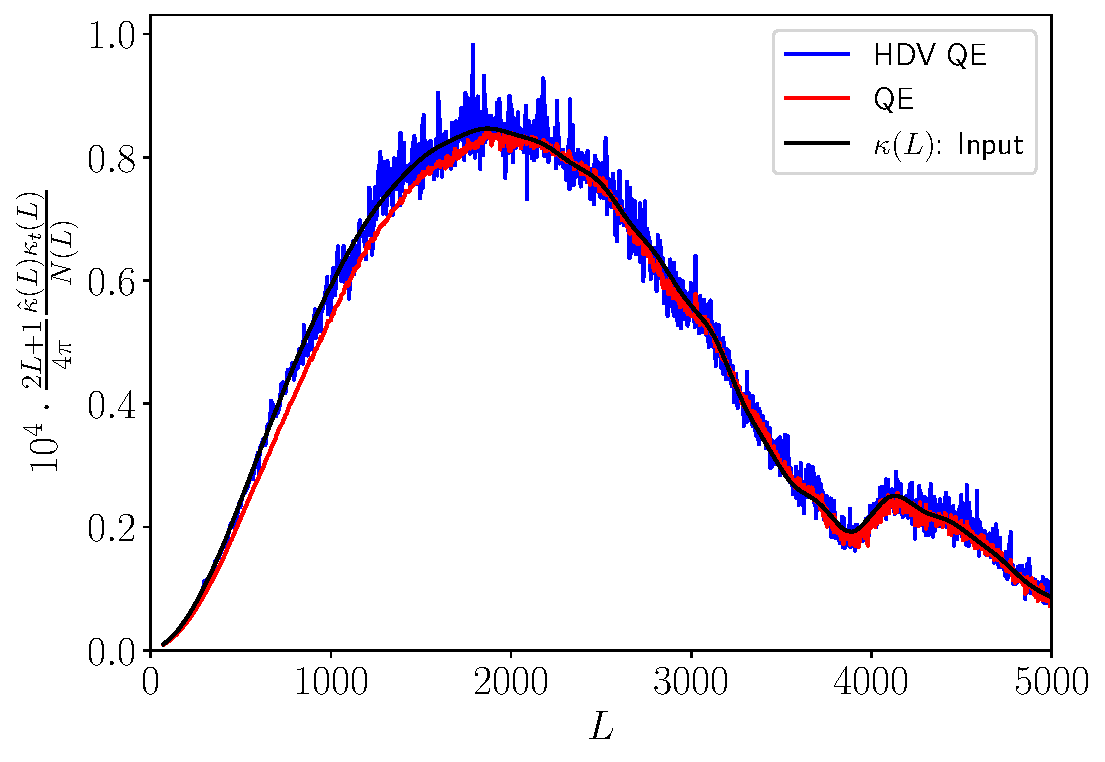
\includegraphics[width=31pc]{Figures/biascomp_M2_lmax4k.pdf}
		\caption{Similar plot as lower panel of Fig. 2 in the paper with $M_{200}=2\times 10^{14}M_{\odot}, l_{\text{max}}=4000$}
	\label{fig1}
\end{figure}

\end{document}